\documentclass[12pt]{article}

\usepackage[english]{babel}
\usepackage{graphicx}
\usepackage[numbers]{natbib}
\usepackage{gitinfo2}
\usepackage{amsmath}
\usepackage[T1]{fontenc}
\usepackage[utf8]{inputenc}
\usepackage{authblk}

\renewcommand\Authands{ and }
\newcommand\tab[1][1cm]{\hspace*{#1}}

\title{A simple statistical model describing burnt area through limitations on fire}

\author[1]{Kelley, Douglas \thanks{\textbf{Email:} douglas.i.kelley@gmail.com
                                   \textbf{Web}: douglask3.github.io}}
\author[2]{Bistinas, Ioannis}
\author[3, 4]{Whitley, R}
\author[1]{Marthews, T}
\author[5, 6]{Burton, C}

\affil[1]{Centre for Ecology and Hydrology\\
          Maclean Building \\
          Crowmarsh Gifford \\
          Wallingford \\
          Oxfordshire \\
          United Kingdom}

\affil[2]{Vrije Universiteit Amsterdam\\
          Faculty of Earth and Life Sciences \\
          Amsterdam \\
          Netherlands}

\affil[3]{Suncorp Group \\
          Personal Lines Pricing Research \\
          Sydney \\
          Australia}

\affil[4]{Macquarie University \\
          Department of Biological Sciences \\
          Sydney \\
          Australia}

\affil[5]{Met Office UK \\
          Exeter \\
          UK}

\affil[6]{Geography \\
          University of Exeter \\
          Exeter \\
          UK}


\begin{document}
\maketitle

\begin{center}
    \textbf{git info}

        git url: https://github.com/douglask3/LimFIRE

	    git revision no: \gitAbbrevHash

        Last commit author: \gitAuthorName,  \gitAuthorEmail

	    Branch: \gitReferences

	    Revision Date: \gitAuthorIsoDate
\end{center}
\newpage

\begin{abstract}

    \textbf{Aim}
    Spatial and temporal patterns of burnt area are controlled by:
        availability of fuel;
        fuel moisture;
        natural and anthropogenic ignitions;
        and anthropagenic suppression.
    Here, we map the limitation and sensitivity of burnt area to each of these controls.

    \textbf{Location}
    Global

    \textbf{Methods}
    We describe a simple framework whereby limitations are imposed by:
        fuel discontinuity;
        fuel moisture and atmospheric drying potential;
        lightning and human ignitions;
        and land use.
    Limitations are described from remote sensed and meteorological observations and optimized against Global Fire Emissions Database (GFED4s) burnt area observations.

    \textbf{Results}
    Fuel moisture is shown to be the main limitation of fire over much of the world, (44\% annual average and 36\% during local dry seasons), particularly in the humid forests and cold, slow drying boreal areas.
    Fuel discontinuity is the next limitation (25\% annually and 23\% in the dry season), especially in deserts and dry season grasslands.
    This is followed by land use change (18\% annually, 21\% dry season)
    and then ignitions (13\% annually, 19\% dry season), which is only a significant limiting factor in dry season savanna,
    where rapid drying of fuel built up during the wet season removes all other natural limitations. In these areas, changes in burnt area are actually more sensitive to other controls, typically land use.

    \textbf{Main conclusions}
    This study contradicts the way basic processes are represented in many global fire models.
    As ignitions only impact burnt area over a limited geographic extent, better representation of controls imposed by fuel loads and moisture is vital. Human ignitions only contribute to a small increase in global burnt area (2%), which is
    offset by the dramatic impact of suppression through anthropogenic land cover changes.
    The assumption
    that humans cause burnt area over much of the world is therefore clearly incorrect, and adequate simulation
    of suppression through land use should become a priority. This result also has implications when considering
    ecosystem services of agricultural land and fire management policies
\end{abstract}


\section{Introduction}

Several studies have examined the global correlation between geographic variability in burnt area and individual potential controls. For example, \citet{bistinas2014causal} used weighted regression to explore the correlation between population density and burnt area. This relationship is unimodal: burnt area initially increases with population density and then decreases. \citet{bistinas2014causal} showed that the location of peak burnt area varied somewhat on different continents and with different types of land use. \citet{van2008climate} compared inter-annual variability in burnt area across the tropics and climate variables related to either fuel accumulation (rainfall in the growing season) or fuel drying (rainfall during the fire season). They showed that increased fire was either correlated with fuel accumulation and anti-correlated with dry season rainfall or vice versa. This suggests that the unimodal relationships of burnt area with factors such as P--E or NPP may be emergent system properties. Thus, in drier areas (which will also have low NPP) fuel availability is the factor limiting the amount of fire; in these regions increasing precipitation leads to increased NPP, increased fuel and hence increased fire. In wetter areas (which will also have higher NPP), fuel is abundant but burning can be limited by fuel wetness; in such areas, increases in rain will further decrease the amount of burning whereas decreases in rain would increase the amount of burning.

\citet{aldersley2011global}, for example, used a regression-tree and random-forest approach to examine the influence of climate, vegetation and human impact on monthly burnt area. They found that climate and vegetation properties were the most important controls on burnt area: for e.g. fires occurred almost exclusively in months with temperatures $>$ 28$^{\circ}$C and the highest burnt areas occurred at precipitation levels between 350-1100mm. Whereas cumulative precipitation and lightning were important variables in determining burnt area, variables related to human impacts were generally unimportant. Gross domestic product (GDP) was the most significant of the human impact variables, but was monotonically and negatively correlated with burnt area. The regression-tree approach initially uses single variable comparisons to construct the branching structure. Thus, while it allows combinations of variables to be considered together, it only partially deals with co-correlation between these variables. Furthermore, the use of variables that display unimodal relationships with burnt area (e.g. Mean Annual Precipitation --- MAP) strongly suggests that these variables are surrogates for the actual controls.

\citet{krawchuk2009global} and \citet{moritz2012climate} used Generalized Additive Models (GAMs) to explore relationships between burnt area and 17 climate variables, NPP and two measures of human impact. Different subsets of the variables were found to be important in different GAMs, but overall NPP (used as a measure of fuel availability) was the most important variable in determining the amount of burning, with variables controlling fuel moisture (in particularly seasonal temperature variables) being the next most important. \citet{moritz2012climate} further demonstrated that the relative importance of specific controls varied geographically and with biome. In the tropics and warm-temperate regions, NPP was the strongest control on the amount of burning in desert, temperate grassland, temperate savanna and Mediterranean ecosystems, whereas factors influencing fuel drying, specifically dry season precipitation and temperature seasonality, were the strongest controls on the amount of burning in tropical and subtropical dry/moist forests.

\citet{knorr2014impact} optimized a non-linear statistical model of fire focusing on the potential human influences on burnt area by using a set of pre-defined but parameterized relationships describing the important natural controls. Thus, they described the influence of fuel production using a positive monotonic relationship between fraction of Absorbed Photosynthetic Radiation (fAPAR) and burnt area, and the influence of fuel dryness using a positive monotonic relationship between the Nesterov Index (NI) and burnt area. They then tested relationships between population density amongst different land cover types/socio-economic development regions and fire frequency (roughly the inverse of burnt area). Using non-linear parameter optimization, they showed that increases in human population result in a significant exponential decrease in fire in all but the most sparsely populated ($<$0.1 people/km\textsuperscript{2}) areas.

\citet{bistinas2014causal} used Generalized Linear Modelling (GLM) to examine the relationships between 11 variables representing vegetation, land use, climate and potential ignition rates (tree cover, grass/shrub cover, NPP, number of dry days, diurnal temperature range, maximum monthly temperature, the ratio of actual to equilibrium evapotranspiration $\alpha$, lightning number, crop area, grazing land area, population density).  The choice of environmental predictor variables was guided by explicit hypotheses about the potential controls of burnt area, and the GLM approach was adopted so as to be able to take account of potential interactions or co-variations between the controls in order to identify the underlying relationships.  \citet{bistinas2014causal} showed that burnt area increases with NPP, number of dry days, maximum monthly temperature, grazing-land area, grass/shrub cover and diurnal temperature range, and decreases with $\alpha$, cropland area and population density. They further showed that there is no significant relationship with the number of lightning strikes or with tree cover. Fuel production (NPP) is the most important determinant of burnt area, with factors affecting the rate of fuel curing (e.g. $\alpha$) and fuel dryness (diurnal temperature range) and fire risk (number of dry days, maximum monthly temperature) next in importance, along with factors that influence fuel type (grass/shrub cover). The simple monotonic relationships between these predictor variables and burnt area are nevertheless sufficient to give rise to complex behavior. Specifically, \citet{bistinas2014causal} show that the unimodal relationships that have been shown between e.g. mean annual temperature, mean annual precipitation, population density and gross domestic product are secondary consequences of correlations among predictor variables. Thus, the unimodal relationship between population density and burnt areas results from the co-variance of population with production and moisture: arid conditions, where fire is limited by productivity and fuel availability, typically support only low population densities.

Thus, a consensus is emerging from these global analyses about the importance of specific controls on fire. All of the studies show that vegetation productivity is the most important control on burnt area, closely followed by factors that influence fuel drying or curing, but with the relative importance of each depending on local environmental conditions. Ignitions, whether natural or anthropogenic appear to be non-limiting to burnt area --- effectively, there are always enough potential fire starts and fire spread is therefore determined by other controls. As demonstrated very clearly by \citet{Knorr2013} and \citet{Bistinas}, the most significant human impact on fire is through suppression with burnt area decreasing with population density.



Coupled vegetation-fire models aim to decribe fire as a function of fuel,moisture and igntions \citep{hantson2016status}
- Humans affact fire in 3 ways:
	1. increased igntions with population and pasture (as incoporated in e.g. SPITFIRE and LmFire)
	1. Fragmentation factor, from crop and urban cover

Knorr et al. 2014 Used fAPAR as fuel idicator. But on sub-annual timestep, this is not fuel load, as dead, non pa vegetation
still contributes to fuel

Similarities to SimFire \citep{knorr2016climate}, but able to test ignitions as well.
Includes postive and negative effects of same variable.


Spatial and temporal patterns of burnt area are controlled by:
    availability of fuel;
    fuel moisture;
    natural and anthropogenic ignitions;
    and anthropagenic suppression.
Here, we map the limitation and sensitivity of burnt area to each of these controls.

%The remainder of this article is organized as follows.
%Section~\ref{previous work} gives account of previous work.
%Our new and exciting results are described in Section~\ref{results}.
%Finally, Section~\ref{conclusions} gives the conclusions.

\section{Methods}

\subsection{Overview}
It is assumed that 100\% burnt area will occur under perfect fire conditions - with full fuel coverage, no moisture, saturated igntions and no agricultural or urban fragmentation. This is analogous to areas in Northern Australia and parts of the sahel which experiance almsot compelet buring each year. Fractional burnt area ($F$) is reduced as each limitation factor ($F_{i}$) becomes sub-optimal, i.e. fuel loads become discontinuous  (e.g. desert areas) or too moist (e.g. Humid evergreen forests), if their is lack of ignition \citep[shown to be an influence inter annual variability in parts Southern Australia][](bradstock2010biogeographic), or with increased human influance on the landscape (e.g. cropland or urban areas).

\begin{equation}
    F=\Pi_{i} F_i
\end{equation}

%\begin{equation}
%    F_i = 1 - l_i
%\end{equation}



\begin{equation}
\begin{split}
    F_{w} = f(w) \\
    F_{\omega} = 1 - f(\omega) \\
    F_{ig} = f(ig) \\
    F_{s} = 1- f(s)
\end{split}
\end{equation}

where
\begin{equation}
    f(x) = (1 + a * e^{-b \cdot x})
\end{equation}


\subsubsection{Fuel ($w$)}

\subsubsection{Moisture ($\omega$)}

\paragraph(Live Fuel)
\citep[$\alpha$ ---  measure of availability of water for plants, and a good index for fuel moisture content ---][]{prentice1993simulation}

\paragraph(Dead Fuel)

\subsubsection{Igntions ($ig$)}

\subsubsection{Supression ($s$)}

\subsection{Analysis}

\subsubsection{Limitation}

\begin{equation}
    \bar{l_{i, X}} = \frac{l_{i, X}}{\sum_{j} l_{j, X}}
\end{equation}

\subsubsection{Sensitivity}

\begin{equation}
    \bar{dl_{i, X}} = \frac{dl_{i, X} \cdot \Pi_{j} l_{j, X}}{l_{i, X}}
\end{equation}

where $dl_{i, X}$ is the gradient of $l_{i, X}$ relative to the maximum possible gradient of $l_{i}$, i.e:

\begin{equation}
    dl_{i, X} = \frac{dl_{i, X} / dx}{dl_{i, l = 0.5} / dx}
\end{equation}

where

\begin{equation}
    \frac{dl_{i}}{dx}
\end{equation}

\begin{figure}[!ht]
  \centering
    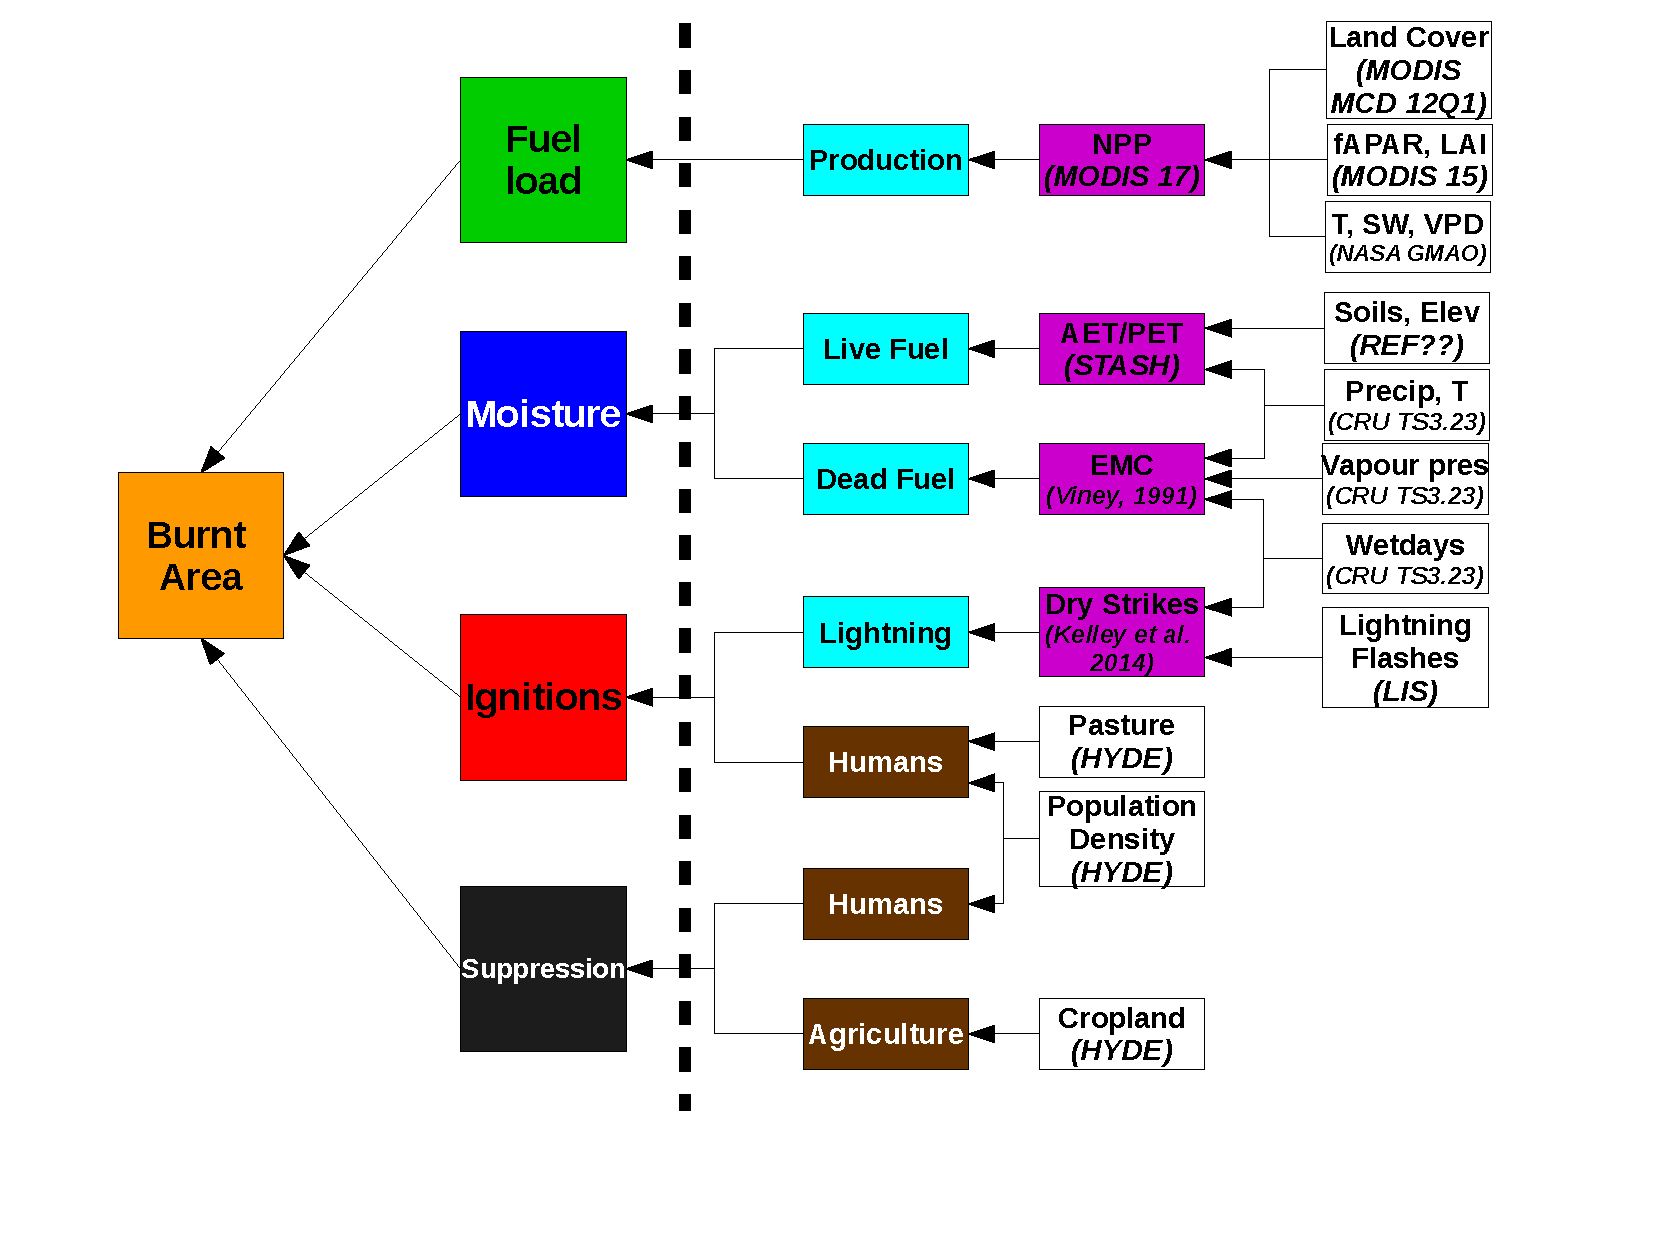
\includegraphics[width=0.67\textwidth]{Model_schematic.pdf}
  \caption{Model description.}
\end{figure}



\section{Results}\label{results}
In this section we describe the results.

\subsection{Benchmarking}

\begin{figure}[!ht]
  \centering
    \includegraphics[width=0.67\textwidth]{../figs/gfedComparison.png}
  \caption{Benchmark comparisons against GFED4s \citep{Giglio2013}.}
\end{figure}

\subsection{Limitations}

\begin{figure}[!ht]
  \centering
    \includegraphics[width=0.67\textwidth]{../figs/limitation_lines.png}

  \caption{Limitation covers.}
\end{figure}


\subsection{Sensitivity}

\begin{figure}[!ht]
  \centering
    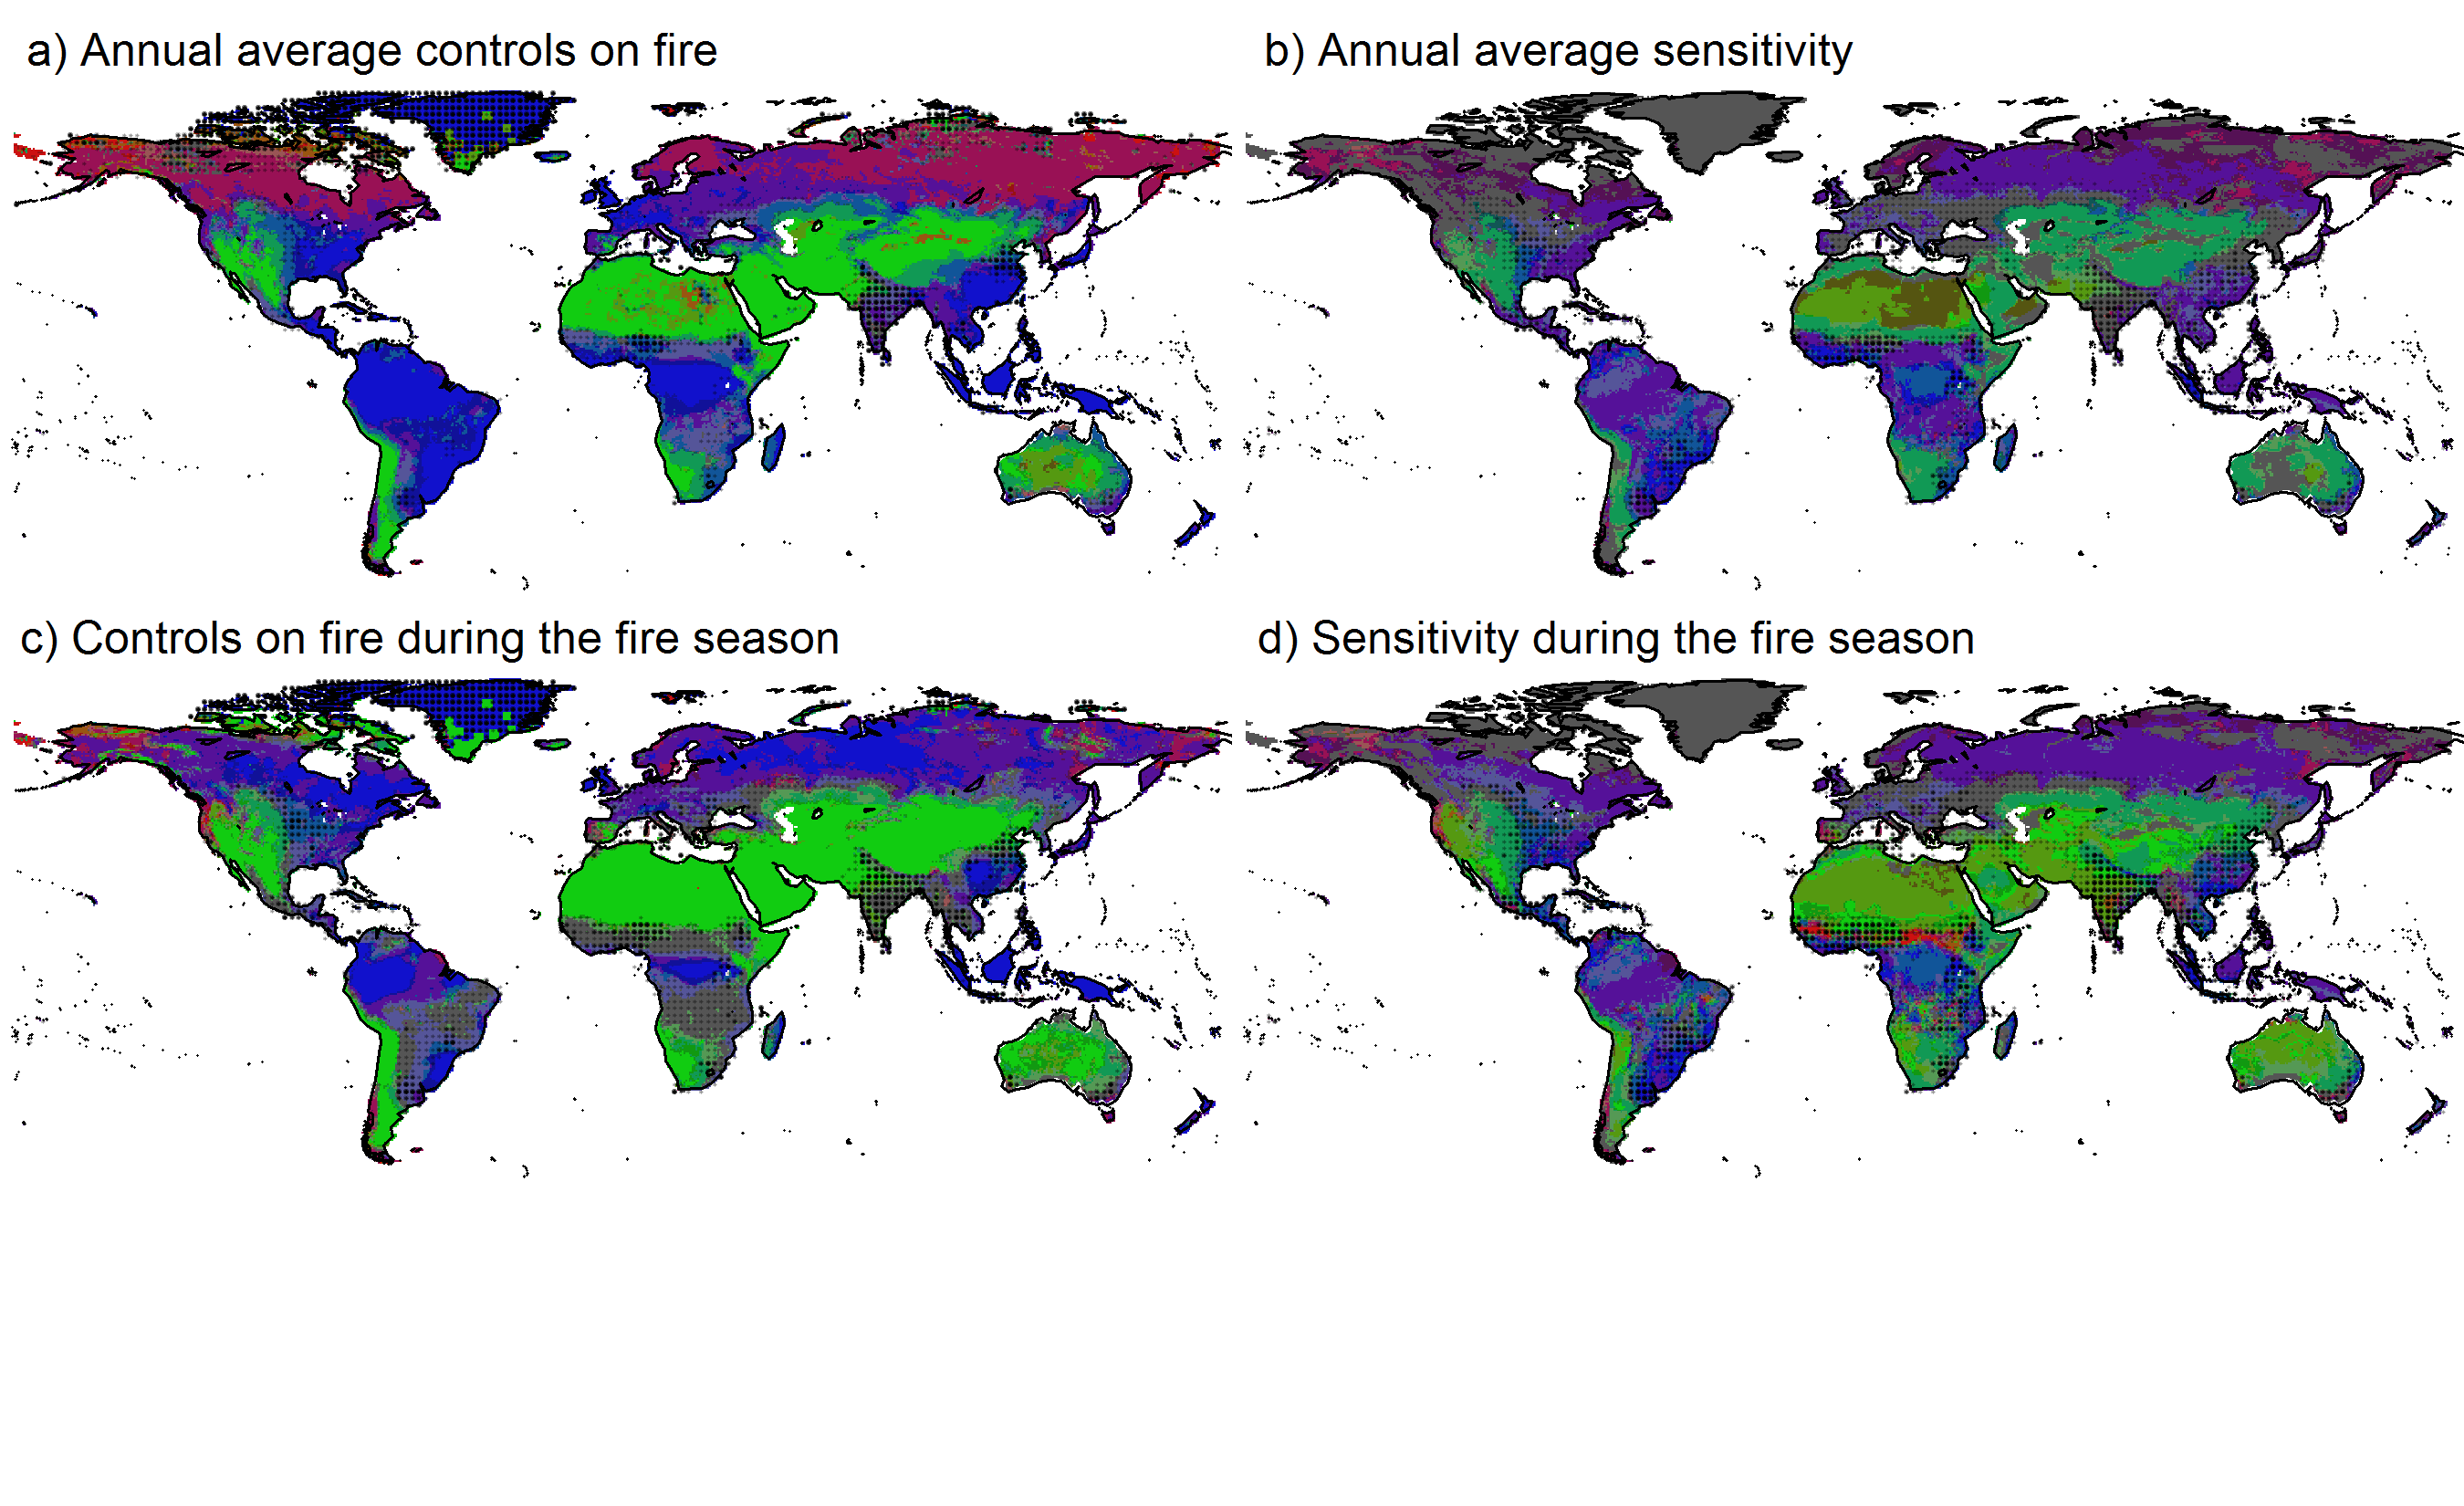
\includegraphics[width=0.67\textwidth]{../figs/limitation_map.png}

  \caption{Limitation and sensitivity.}
\end{figure}

\section{Conclusions}\label{conclusions}

\section{Papers and Applications}

\subsection{What limits fire, where and when: sensitivity of burnt area to different controls}

\subsubsection{Abstract}
Global fire models typically describe fire as a consequence of fuel load, moisture, natural and anthropogenic
ignitions, and land use suppression. A lack of information on the temporal and spatial distribution of these
controls has meant that their simulated effects on predicting burnt area are largely untested. Despite this,
there is a pervasive assumption that burnt area is proportional to the number of ignitions, with many models
predicting significant increases in burnt area with human fire starts.


Here, we map the limitation and sensitivity of burnt area to each control using a simple framework whereby
limitations are imposed by: fuel discontinuity; fuel moisture and atmospheric drying potential; lightning and
human ignitions; and land use. Limitations are described from remote sensed and meteorological
observations and optimized against Global Fire Emissions Database (GFED4s) burnt area observations.
Fuel moisture is shown to be the main limitation of fire over much of the world, (44\% annual average and
36\% during local dry seasons), particularly in the humid forests and cold, slow drying boreal areas. Fuel
discontinuity is the next limitation (25\% annually and 23\% in the dry season), especially in deserts and dry
season grasslands. This is followed by land use change (18\% annually, 21\% dry season) and then ignitions
(13\% annually, 19\% dry season), which is only a significant limiting factor in dry season savanna, where
rapid drying of fuel built up during the wet season removes all other natural limitations. In these areas,
changes in burnt area are actually more sensitive to other controls, typically land use.


This study contradicts the way basic processes are represented in many global fire models. As ignitions only
impact burnt area over a limited geographic extent, better representation of controls imposed by fuel loads
and moisture is vital. Human ignitions only contribute to a small increase in global burnt area (2\%), which is
offset by the dramatic impact of suppression through anthropogenic land cover changes. The assumption
that humans cause burnt area over much of the world is therefore clearly incorrect, and adequate simulation
of suppression through land use should become a priority. This result also has implications when considering
ecosystem services of agricultural land and fire management policies.

\pagebreak
x
\pagebreak
\subsection{Anthropagenic regime shifts}
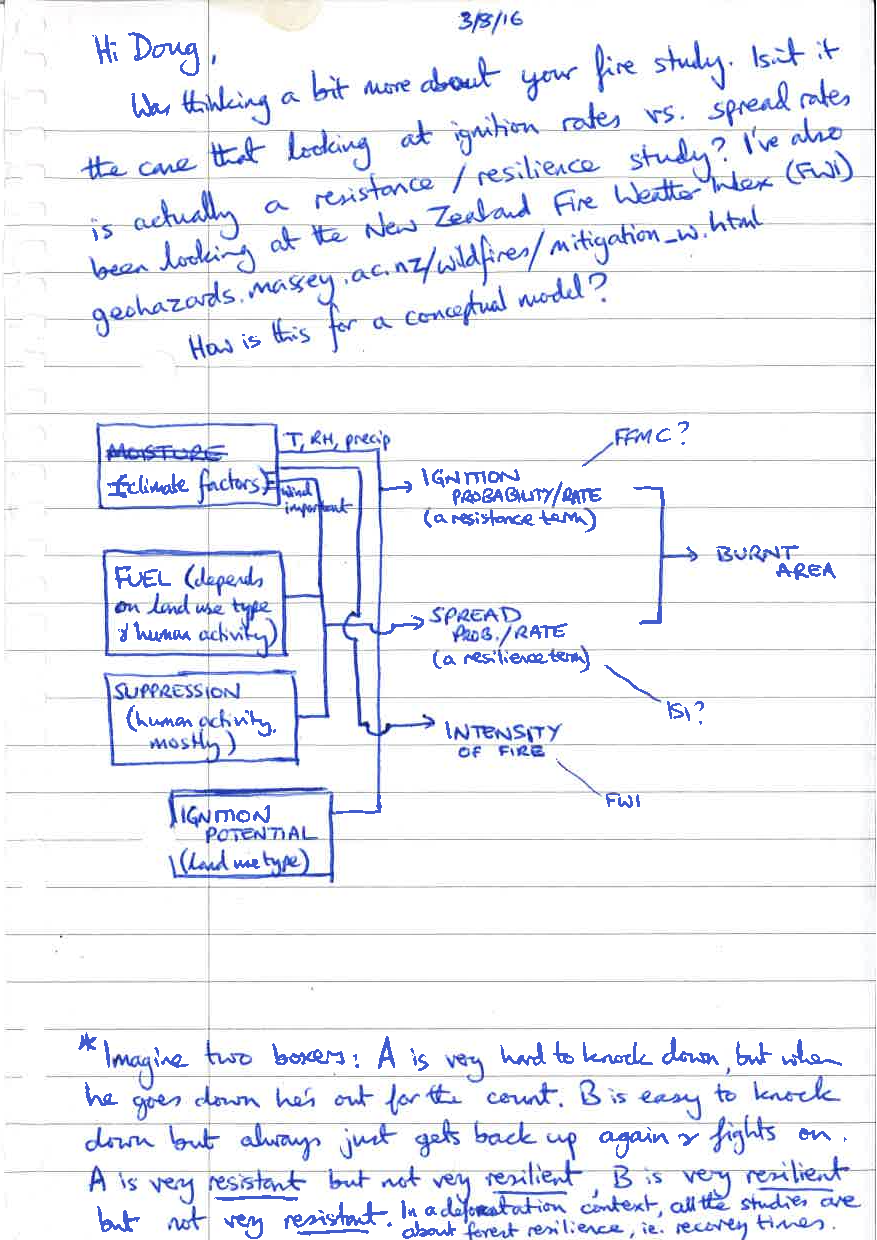
\includegraphics[width=0.99\textwidth]{tobys_notes.pdf}

\bibliographystyle{plainnat}
\bibliography{Model_description}

\end{document}
This is never printed
